% ┌                                                ┐
% │     AUTHOR: Janis Hutz<info@janishutz.com>     │
% └                                                ┘

% Lecture: Wir besitzen nicht das komplette Vorwissen in der Analysis für dieses Kapitel, d.h. wird totales Verständnis nicht 
%
% Lecture: Intuitiv wird Fourier-Trans. zur Kompression genutzt, z.b. jpg format.
\subsection{Fourier-Reihen}
Eine Anwendung der Schnellen Fourier-Transformation (FFT) ist die Komprimierung eines Bildes und sie wird im JPEG-Format verwendet.

\fancydef{Trigonometrisches Polynom von Grad $\leq m$} Die Funktion:
\rmvspace
\begin{align*}
    p_m(t) := t \mapsto \sum_{j = -m}^{m} \gamma_j e^{2 \pi ijt} \text{ wobei } \gamma_j \in \C \text{ und } t \in \R
\end{align*}
%
%
\inlineremark $p_m : \R \rightarrow \C$ ist periodisch mit Periode $1$.
Falls $\gamma_{-j} = \overline{\gamma_j}$ für alle $j$, dann ist $p_m$ reellwertig und
% NOTE: Uhh... do we want to use the fancy symbols for real and imaginary part or just use $\text{Re}$?
% RESPONE: whatever he uses in the script, preferably \text{Re}() etc.
$p_m$ kann folgendermassen dargestellt werden ($a_0 = 2\gamma_0, a_j = 2\Re(\gamma_j)$ und $b_j = -2\Im(\gamma_j)$):
\rmvspace
\begin{align*}
    p_m(t) = \frac{a_0}{2} + \sum_{j = 1}^{m} (a_j \cos(2\pi jt) + b_j \sin(2\pi jt))
\end{align*}

\begin{definition}[]{$L^2$-Funktionen}
    Wir definieren die $L^2$-Funktionen auf dem Intervall $(0, 1)$ als
    \rmvspace
    \begin{align*}
        L^2(0, 1) := \{ f: (0, 1) \rightarrow \C \divides ||f||_{L^2(0, 1)} < \infty \}
    \end{align*}
    während die $L^2$-Norm auf $(0, 1)$ durch das Skalarprodukt
    \rmvspace
    \begin{align*}
        \langle g, f \rangle_{L^2(0, 1)} := \int_{0}^{1} \overline{g(x)} f(x) \dx x
    \end{align*}
    über $||f||_{L^2(0, 1)} = \sqrt{\langle f, f \rangle_{L^2(0, 1)}}$ induziert wird
\end{definition}

\inlineremark $L^2(a, b)$ lässt sich analog definieren mit
\rmvspace
\begin{align*}
    \langle g, f \rangle_{L^2(a, b)} & := \int_{a}^{b} \overline{g(x)} f(x) \dx x                              \\
                                     & = (b - a) \int_{0}^{1} \overline{g(a + (b - a)t)} f(a + (b - a)t) \dx t
\end{align*}
In Anwendungen findet sich oft das Intervall $\left[ -\frac{T}{2}, \frac{T}{2} \right]$.
Dann verwandeln sich die Integrale in die Form $\frac{1}{T} \int_{\frac{T}{2}}^{-\frac{T}{2}} (\ldots) \dx t$ und $\exp(2\pi ijt)$ durch $\exp(i \frac{2\pi j}{T} t)$ ersetzt wird.

\stepcounter{all}
\inlineremark Die Funktionen $\varphi_k(x) = \exp(2\pi ikx)$ sind orthogonal bezüglich des $L^2(0, 1)$-Skalarprodukts, bilden also eine Basis für den Unterraum der trigonometrischen polynome.


\inlinedef Eine Funktion $f$ ist der $L^2$-Grenzwert von Funktionenfolgen $f_n \in L^2(0, 1)$, wenn für $n \rightarrow \infty$ gilt, dass $||f - f_n||_{L^2(0, 1)} \rightarrow 0$


\begin{theorem}[]{Fourier-Reihe}
    Jede Funktion $f \in L^2(0, 1)$ ist der Grenzwert ihrer Fourier-Reihe:
    \rmvspace
    \begin{align*}
        f(t) = \sum_{k = -\infty}^{\infty} \hat{f}(k) e^{2\pi ikt}
    \end{align*}
    wobei die Fourier-Koeffizienten
    \rmvspace
    \begin{align*}
        \hat{f}(k) = \int_{0}^{1} f(t)e^{-2\pi ikt} \dx t \smallhspace k \in \Z
    \end{align*}
    definiert sind. Es gilt die Parseval'sche Gleichung:
    \rmvspace
    \begin{align*}
        \sum_{k = -\infty}^{\infty} |\hat{f}(k)|^2 = ||f||_{L^2(0, 1)}^2
    \end{align*}
\end{theorem}
\inlineremark Oder viel einfacher und kürzer: Die Funktionen $\varphi_k(x)$ bilden eine vollständige Orthonormalbasis in $L^2(0, 1)$.

% A (small) intuitive explanation of what the fourier series / coefficients are & what they are useful for would be great, script *briefly* touches on it.

\setcounter{all}{14}
\inlineremark Die Parseval'sche Gleichung beschreibt einfach gesagt einen ``schnellen'' Abfall der $\hat{f}(k)$.
Genauer gesagt, klingen die Koeffizienten schneller als $\frac{1}{\sqrt{k}}$ ab.
Sie sagt zudem aus, dass die $L^2$-Norm der Funktion aus einer Summe berechnet werden kann (nicht nur als Integral).
Wenn wir die Fourier-Reihe nach $t$ ableiten, erhalten wir
\rmvspace
\begin{align*}
    f'(t) = \sum_{k = -\infty}^{\infty} 2\pi ik\hat{f}(k)e^{2\pi ikt}
\end{align*}

\begin{theorem}[]{Fourier-Reihe}
    Seien $f$ und $f'$ integrierbar auf $(0, 1)$, dann gilt $\hat{f'}(k) = 2\pi ik\hat{f}(k)$ für $k \in \Z$.

    Falls die Operationen erlaubt sind, dann gilt zudem:
    \rmvspace
    \begin{align*}
        \hat{f^{(n)}} = (2\pi ik)^n \hat{f}(k) \text{ und } ||f^{(n)}||_{L^2}^2 = (2\pi)^{2n} \sum_{k = -\infty}^{\infty} k^{2n} |\hat{f}(k)|^2
    \end{align*}
\end{theorem}


\inlinetheorem Wenn $\displaystyle \int_{0}^{1} |f^{(n)}(t)|\dx t < \infty$, dann ist $\hat{f}(k) = \tco{k^{-n}}$

Falls die Funktion jedoch nicht glatt ist, dann entstehen \textit{Überschwingungen} an den Sprungstellen, die näher und näher an die Sprünge herankommen, aber nicht kleiner werden, wenn wir mehr Terme der Fourier-Reihe aufsummieren.
Das Phänomen wird das \bi{Gibbs-Phänomen} gennant und wir haben $L^2$-Konvergenz, aber keine punktweise Konvergenz an der Sprungstelle.

\inlineremark
Diese Überschwingungen entstehen durch die Definition der Fourier-Reihe und sind in der untenstehenden Abbildung \ref{fig:trigo-interp-overarcing} aus dem Skript sehr gut ersichtlich.
Die dargestellte Funktion ist die Fourier-Reihe der charakteristischen Funktion des Intervalls $[a, b] \subseteq ]0, 1[$, welche sich folgendermassen analytisch berechnen lässt:
\begin{align*}
    b - a + \frac{1}{\pi} \sum_{k \neq 0} e^{-ikc}\frac{\sin(kd)}{k} e^{i2\pi kt}, \mediumhspace t \in [0, 1]
\end{align*}
Mit $c = \pi(a + b)$ und $d = \pi(b - a)$

% TODO: Replace with rendered image from matplotlib (will be higher quality than screenshot from script and can tweak it to our liking)
% we will have it anyway after solving the exercises, so might as well
\begin{figure}[h!]
    \begin{center}
        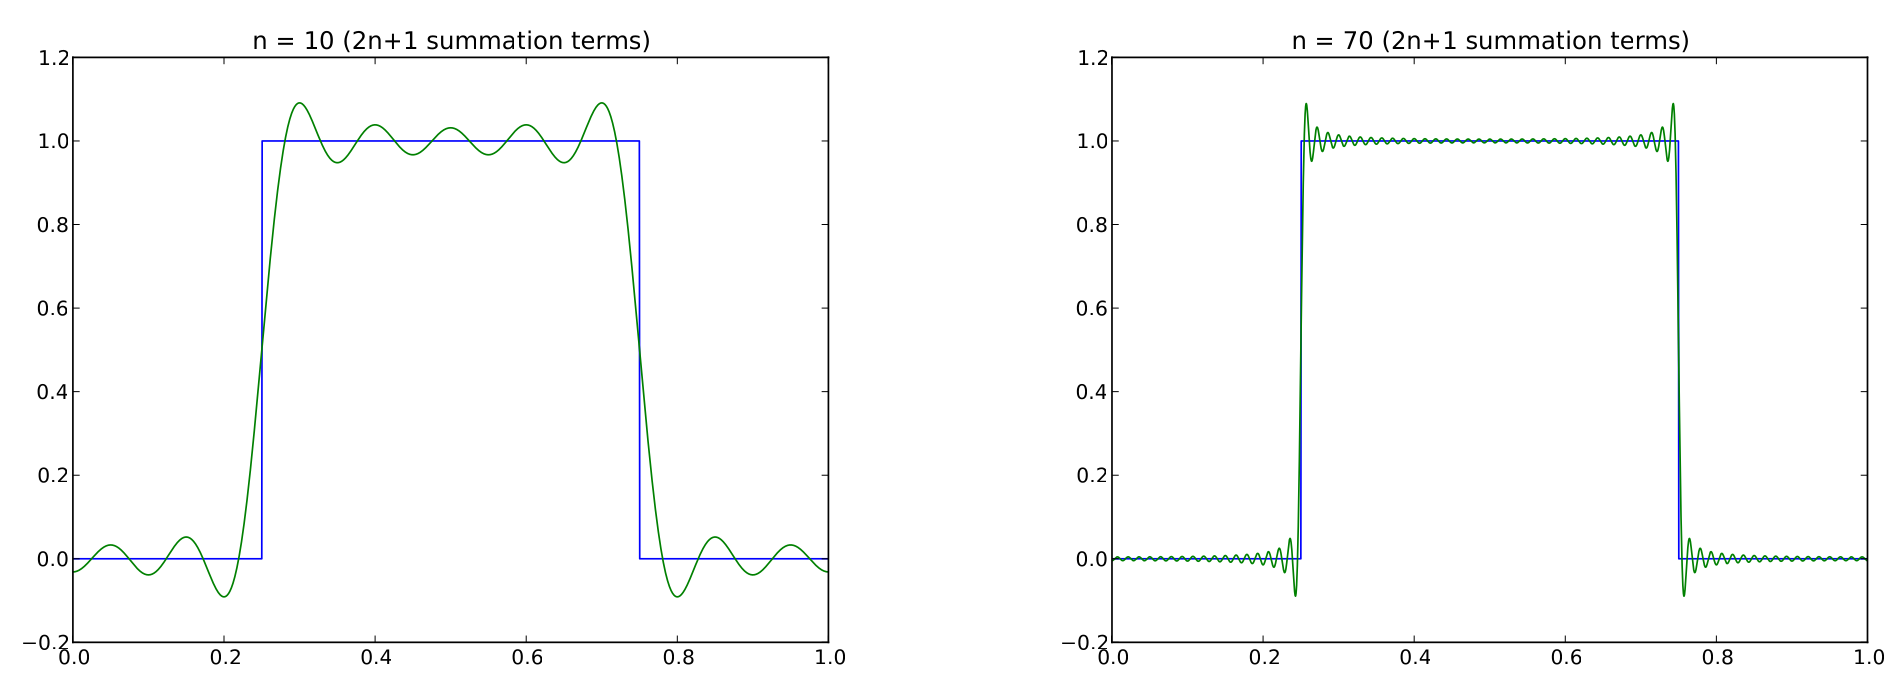
\includegraphics[width=0.95\textwidth]{assets/01_interpolation/01_trigonometric/overarcing.png}
    \end{center}
    \caption{Überschwingungen der Fourier-Reihe der charakteristischen Funktion des Intervalls $[a, b] \subseteq ]0, 1[$.
    (Abbildung aus dem Vorlesungsdokument von Prof. V. Gradinaru, Seite 69)}
    \label{fig:trigo-interp-overarcing}
\end{figure}

\stepcounter{all}
\inlineremark Meist ist es nicht möglich (oder nicht sinnvoll) die Fourier-Koeffizienten analytisch zu berechnen,
weshalb man wieder zur Numerik und der Trapezformel greift, die folgendermassen definiert ist für $t_l = \frac{l}{N}$,
wobei $l = 0, 1 \ldots, N - 1$ und $N$ die Anzahl der Intervalle ist:
\begin{align*}
    \hat{f}_N(k) := \frac{1}{N} \sum_{l = 0}^{N - 1} f(t_l) e^{-2\pi ikt_l} \approx \hat{f}(k)
\end{align*}

% TODO: Consider if we should use the below

% \begin{tikzpicture}
%     \begin{axis}[
%         legend pos=outer north east,
%         title=Function plot of $f(x)$ (parts coloured),
%         axis lines = box,
%         xlabel = $x$,
%         ylabel = $y$,
%         variable = t,
%         trig format plots = rad,
%     ]
%         \addplot [
%             domain=1:4,
%             samples=70,
%             color=blue,
%         ]
%         {log2(x)};
%         \addlegendentry{$ y=x^2 - x - 0.5$}
%     \end{axis}
%     \node (0) at (0, 0) {};
% \end{tikzpicture}

